\section{Vertex Detectors}

\begin{figure}
    \centering
    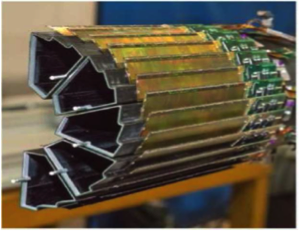
\includegraphics[width=.5\linewidth]{Spinoffs/STAR.png}
    \caption{Pixel detector for the STAR experiment}
    \label{fig:spinoffs:star}
\end{figure}

\begin{figure}
    \centering
    \includegraphics[width=.5\linewidth]{Spinoffs/BelleII_Depfet.png}
    \caption{A DEPFET ladder for the Belle II vertex detector}
    \label{fig:spinoffs:belleII}
\end{figure}

\subsection{CMOS}
CPS developed at IPHC in perspective of the ILC are used in several
devices, as illustrated by the non-exhaustive list below:
\begin{itemize}
\item Several high precision transparent beam telescopes, adapted to
	($<\unit[1]{GeV}$) electron beams, are equipped with the MIMOSA-26 or
	-28 (alias ULTIMATE) sensors
\item The first generation of sensors with full on-chip signal processing
	developed at IPHC (in a $\unit[0.35]{\mu m}$ CMOS process) was applied to the
	STAR-PXL detector at RHIC, which completed successfully its first
	data campaign in 2014 and has started its 2015 run
\item The upgraded ALICE ITS will be the next equipment based on CPS;
	it will provide insight of a token ring architecture pioneering
	the one considered for the IBISCUS chip mentioned above; it will
	also provide running experience with a tracker based on CPS
\item The Micro-Vertex Detector of the CBM experiment at FAIR/GSI will
	also be based on the CPS presently developed for the ALICE-ITS
	upgrade
\item The sensors were, or are, being applied outside of subatomic physics.
	They were for instance used in the FIRST experiment at GSI, for
	hadrontherapy monitoring; they are presently developed for soft
	X-Ray imaging and brain-imaging.
\end{itemize}

Sensors featuring pixels about 5 times larger than those equipping the STAR-PXL were fabricated in 2014, with different pixel design optimisations. Such large pixels are more exposed to the effects of signal charge recombination. The purpose of the paper is, among others, to show that the charge particle detection efficiency is not degraded, even after radiation loads representative of upcoming trackers, such the upgraded ALICE Inner Tracking System. The charged particle detection performances of these large pixel CPS prototypes with integrated signal processing and binary outputs were studied by exposing the sensors to a 450 MeV electron beam. The results obtained will be exposed
and shown to validate the concept for its evolution towards large area tracking devices, with the perspective of integrating logical strips in the sensor.

\subsection{DEPFET}
The concept of a DEPFET active pixel detector for vertex detection at collider experiments was initiated in the linear collider community (for TESLA). The election of DEPFET technology for the Belle II detector therefore represents an important spin-off of linear collider detector R\&D. DEPFET is also considered a strong candidate technology for the vertex detector at a future circular collider (http://cepc.ihep.ac.cn/preCDR/volume.html). DEPFET detectors are furthermore used for X-ray imaging at the XFEL~\cite{xfel}. Future space missions envisage the use of DEPFET sensors~\cite{bepicolombo}. Their use in microscopy is being studied.

\subsection{FPCCD}
    Because of the relatively slow readout speed, the application of FPCCD sensors to other high energy physics experiments would be limited. However, high spatial resolution of small pixel size must be applicable to measurements of X-ray imaging.
    Two-phase \ce{CO2} cooling system can be applied to any other detectors which require efficient cooling between \unit[-40]{\degree C} and near room temperature. Our system, which uses a \ce{CO2} gas compressor, has a great advantage for low temperature operation near \unit[-40]{\degree C} compared with systems using liquid pumps for circulation.

\subsection{Chronopix}
     With some modifications (for example, adding time-time converter) ChronoPixel architecture can be applied for any experiment requiring time stamping of individual hits -- it may be HL-LHC, CLIC and so on.

\subsection{SOI}

\subsection{3D Pixel Development}
As stated above the technology is already being developed for CMS and x-ray imaging applications.  The large area sensor concept is applicable for a variety of focal plane array concepts.

\subsection{CLICpix}
The CLIC vertex-detector R\&D shares its main challenges of simultaneously achieving small pixel pitch,
low material budget and fast timing with other future pixel detector projects, such as the developments for
the upgrades of the LHC detectors for high-luminosity operation or for future circular colliders.
Synergies with these projects are exploited for example in the context of the RD53 collaboration for \unit[65]{nm} hybrid readout
ASICs~\cite{RD53} and via the AIDA2020 project for Advanced European Infrastructures for Detectors at
Accelerators~\cite{AIDA2020}.
Moreover the CLICpix ASIC is derived from the
Timepix/Medipix family of hybrid readout ASICs~\cite{medipix-collaboration}, which have a wide range of applications in
medical imaging and material science.

\section{Silicon Tracking}
\subsection{Long-Ladder and Charge Division Tracking R\&D}

It should be noted that the exploration of noise limitations for long, thin electrodes apply independently
of the sensor technology that generates the signals. Thus, this work may have
relevance to detection issues across a wide array of fields.

\subsection{Resistive charge-division on thinned micro-strips sensors with low signal amplification}
The application of LGAD devices to the LC tracking is a spin-off of its original aim as timing devices for high radiation environments, this technology is being proposed as vertex locator technology for the LHC experiments: AFP2 and HGTD (ATLAS); and CT-PPS (CMS)~\cite{Sadrozinski:CPAD2015}.

\subsection{KPIX}
This work represents a significant step in the aggressive integration of silicon sensors with readout electronics, just short of integrating the electronics directly into the sensors. It has prompted consideration of this approach by CMS for calorimetry and by ATLAS for a muon system.  It may have applications in sensors for light sources as well as other particle physics detectors.

\section{Gaseous Tracking}
\subsection{Resistive Micromegas}
The ND280 TPC at KEK uses the technology developed for ILC.
A strong effort is pursued to develop detectors with similar technology for other applications such as
the study of low energy neutrinos and the search for Dark Matter.
Several TPCs for Nuclear Physics experiments are based on these developments. They are specifically discussed in a
conference held every two years in Paris~\cite{Irastorza:2013mxa}.

\subsection{Pixelized Readout}
A single GridPix detector is taking data for more than 1 year in the CAST
experiment for axion search.
For the LHCb VELO upgrade project a particle tracking telescope was constructed
based on the Timepix-3 ASIC.
In collaboration with KVI-CART in Groningen (NL) a system for proton radiography
is being developed using small (gaseous) TPCs based on GridPix detectors, for
accurate 3D proton tracking.

\subsection{InGrid}
A single InGrid detector will be installed this year in the CAST experiment for axion search. For a TPC in a CLIC detector, a highly granular (i.e. pixelized) readout structure is mandatory to lower the occupancy.

\subsection{Electronics, DAQ and Cooling}
The front end electronics, based on the SALTRO16-chip provides a very versatile system in the sense that it offers the possibility to set various readout parameters (polarity, shaping time, gain, decay time) in the SALTRO pre-amplifier. It is optimized for low capacitance detectors, sensitive to femtocoulomb signals with digital correction of the base line, followed by advanced pulse recognition and zero suppression.  In that sense the SALTRO-chip can be regarded as a highly sensitive 16 channel digital oscilloscope. The small units of the readout system are suitable for applications and detector R\&D in a variety of other fields like medical diagnostics, material science at XFEL, and for investigations at ESS.

\section{Calorimetry}
\subsection{Scintillator Strips}
\begin{itemize}
	\item photo-sensor named MPPC from Hamamatsu Photonics KK is employed for the T2K experiment, CMS upgrade (HC-CAL), Belle II detector (end-cap muon)
	\item PET and SPECT development
\end{itemize}

\subsection{Silicon-Tungsten ECAL in ILD}
\begin{itemize}
\item CMS phase-2 upgrade project of the
 endcap calorimetry (HGCAL).
\item The compact Silicon-W design has been used in the PAMELA satellite (very
 similar to the CALICE SiW ECAL physics prototype)~\cite{1742-6596-160-1-012039}.
\item Future circular $e^+e^-$ high energy colliders (FCC in CERN, CEPC in China)
may also use this technology.
\end{itemize}

\subsection{Silicon Tungsten SiD ECAL}
This work represents a significant step in the aggressive integration of silicon sensors with readout electronics, just short of integrating the electronics directly into the sensors. It has prompted consideration of this approach by CMS for calorimetry and by ATLAS for a muon system.  It may have applications in sensors for light sources as well as other particle physics detectors.

\subsection{DHCAL}
The DHCAL technology was specifically developed for the hadron calorimeter of the ILC, with its low particle rate and radiation dose. To export the technology to other environments, the rate capability of the chambers and the radiation hardness of the readout need to be improved. The former is being addressed with low-resistivity plates (glass and Bakelite), while the latter will require a new front-end readout system based on an ASIC using a smaller feature size. Possible applications are the tail catcher of the forward calorimeters of CMS and the outer wheels of the ATLAS muon system. Both options are being pursued actively.

\subsection{GEM}
This technology is already being used in many areas of application: CMS forward chambers, planar chambers for TOTEM, and even in cylindrical geometries. Beyond HEP, GEM technology is used in many in many human and animal medical imaging systems, and in muon tomography for homeland security. Many applications can be found at the CERN RD51 web site and links to RD51 meetings therein~\cite{RD51Collaboration}.

\subsection{THGEM-based sampling elements for DHCAL}
So far, our studies of THGEM-based detectors, particularly the RPWELL, have yielded a cost-effective, single-stage completely stable device, with wide dynamic range. The RPWELL concept is suitable for a variety of applications that do not require very high spatial and energy resolutions. Current examples are CsI-coated multipliers for UV-photon imaging in RICH detectors; cryogenic gaseous photomultipliers for recording scintillation-light in noble-liquid detectors, developed for future dark-matter and neutrino experiments, medical imaging and in combined neutron/gamma inspection systems; fast-neutron detectors with dedicated converter-foils and Muon tomography inspection systems for the detection of hazardous materials in cargo.

\subsection{Dual Readout}
High precision calorimetry is vital to many experiments, both collider and fixed target; dual-readout is considered for a space station experiment; and, a high-precision dual-readout calorimeter is being considered for an electron -- ion collider.

\subsection{FCAL}
The expertise acquired within FCAL for radiation hard sensors and fast front-end electronics was
used to build, commission and operate fast
beam-conditions monitors at the CMS experiment at LHC.
Radiation hard sensors developed within FCAL are used as beam-loss monitors
with excellent time resolution at FLASH, XFEL and LHC.
In addition, front-end ASICs are under development for the upgrade of the LHCb tracker.

\section{Muon System}
\subsection{Scintillator/Silicon Photomultiplier}
The development of the Digital SiPMs will have strong impact on the many application areas

One of the important application of practically full design and technology of the Muon /Tail Catcher System in the Homeland Security is the Muon Tomography for the security checking of the transport containers. The checking of the millions of the transport container in present time is one of the crucial and urgent problems, which don't have the efficient solution. The muon tomography, based on the HEP Muon System could be solution.

The development of the Digital SiPMs will have strong impact in Nuclear Medicine, in particular development of  Positron Emission Tomography (PET).  The new generation of the PET scanners will be developed on base of the All Digital SiPM Readout with more advanced performance.

\section{AIDA-2020 for LC experiments}
AIDA-2020 is a research initiative funded by the European Union to advance the development of infrastructures for research on detectors for accelerator experiments. It runs from 2015 to 2019 and unites 38 beneficiaries from 19 countries. The total budget amounts to 29 MEUR, including 10 MEUR of direct support from the EU. The program is aligned with the European strategy for particle physics; thus about 50\% of the activities are motivated by the needs of LHC detector upgrades, but there is a significant fraction of about 25\% targeted at linear collider experiments.

AIDA-2020 follows the successes of the previous initiatives EUDET and AIDA. The infrastructure theme, although interpreted in a wider sense, moves common interests of R\&D groups into focus and helps structuring the activities. It builds on the achievements of EUDET and AIDA, e.g. test beam infrastructures like the TPC magnet, the pixel telescopes or software frameworks like DD4HEP, but it goes beyond in many respects. There is a three times larger budget to directly support users of, e.g., test beams, and there are new topics, like novel silicon sensors and micro-channel cooling.

Efforts, with strong representation of LC groups, will enhance infrastructures to advance towards the construction phase of calorimeters and gaseous detectors. This includes test stands for the characterization of silicon sensors or optical read-out units for highly granular calorimeters, as well as installations for the production and characterization of large area gas detectors, RPCs, GEMs, and micromegas,. Test beam infrastructure is further improved, to keep pace with increased demands of precision detectors, e.g. by adding a silicon strip telescope to the TPC test stand at the DESY.

Development of micro-electronic ASICs directly supports the efforts in vertex detector, tracking and calorimeter R\&D. Particular attention, and a special fund, is devoted to the cooperation with industry and the transfer of technologies, e.g. for the production of large areas of silicon devices. Work on advanced software is strongly driven by LC needs and includes work on tracking tools and particle flow algorithms (PandoraPFA). The LC community had assigned high priority, in the proposal preparation phase, to the creation of a common DAQ framework for test beam experiments of several linear collider sub-detector prototypes in a combined set-up, which is now being pursued in a dedicated work package.

While activities remain coordinated in the R\&D collaborations, AIDA-2020 represents a unique forum for intensive exchange between LHC and LC communities united in common working groups. This matches well the move of focus towards precision on the LHC side as well as to realistic detector designs in the LC world.
